%!TEX root = thesis.tex
\chapter{2-D Imaginary Time Evolving Block Decimation}
\label{chapter:2ditebd}
In this chapter, we disscues how to generalize the 1D-iTEBD algorithms to 2D and how to further improve the method.
%In one-dimensional many-body states, the performance of one-dimension imaginary time evolving block decimation (1D-iTEBD) is very well, especially its high efficiency. It is straightforward to think of expanding this framework to two-dimensional problems. However, through many attempts we notice that the accuracy in 2-D is less than 1-D. In order to overcome that obstacle, optimization of 2-D algorithms becomes an significant issue in condense matter physics. 

In Sec.~\ref{ite} and Sec.~\ref{itebd}, we briefly review the idea of imaginary time evolution (TEBD) \cite{PhysRevLett.93.040502} \cite{PhysRevB.78.155117} and explain how to extend it to simulate an infinite two-dimensional system (2D-iTEBD) \cite{PhysRevB.86.195137}. However, the method presented in Ref.~\cite{hahaPhysRevB.86.195137} is unstable because it multiplies too many pseudo-inverse matrices during the update of the wave-functions. Hence, In Sec.~\ref{2dhastin} and Sec.~\ref{2dopt} we will discuss the improvement of 2D-iTEBD in detail, such as the method developed by Hastings \cite{light_hastings}, splitting projection states by QR and LQ decomposition, etc. In Sec.~\ref{Comparison}, we utilize 2D-iTEBD to simulate the Heisenberg and transverse Ising models on two-dimensional square lattice and compare the features among 2D-iTEBD algorithms implemented with different strategies.


\section{Imaginary Time Evolution}
\label{ite}
Theoretically, we could project any initial random states to the ground state if the imaginary time evolution operator $e^{-\tau H}$ exists,  
\begin{align}
	\label{mapgroud}
	\Ket{\psi_0} = \frac{e^{-\tau H} \Ket{\Psi}}{\parallel e^{-\tau H} \Ket{\Psi}\parallel}
\end{align}
where $H$ is the Hamiltonian of a specific model. However, according to Eq.~(\ref{wavefunc}), we have known that the number of coefficients the evolution operator $e^{-\tau H}$ is proportional to $d^N \times d^N$. In other words, it is impossible to update entire system directly. Therefore, in one-dimensional quantum many-body systems we apply MPS structure to restrict the exponential increase of the dimension. 

In order to update the two tensors in the unit cell [Fig.~\ref{fig312}], we utilize the \textit{Suzuki-Trotter decomposition} to approximate the entire evolution operator with $2$-sites operators. \textit{The first-order Suzuk-Trotter decompostio} of operator $e^{\delta (A+B)}$ is,
\begin{align}
	\label{STd}
	e^{\delta A + B} = e^{\delta A}e^{\delta B} + O(\delta^2)
\end{align}
where $A$ and $B$ are two non-commutative operators.Therefore, the entire evolution operator can be approximated by grouping the two site operator as $H_{AB}$ and $H_{BA}$,
\begin{align}
	\label{evoopt}
	e^{-\tau H} = \left(e^{-\delta H}\right)^{\frac{\tau}{\delta}} \approx \left(\prod e^{\delta H_{AB}} \right)\left( \prod e^{\delta H_{BA}}\right)
\end{align}
and we can obtain the evolution operator $e^{H_{AB}}$ and $e^{H_{BA}}$ straightly after solving two-site Hamiltonians, $H_{AB}$ and $H_{BA}$.
So far, we have constructed the infinite MPS and the 2-site evolution operators $e^{-\tau H_{AB}}$ and $e^{-\tau H_{BA}}$. The tensor network representation of Eq.~\ref{mapgroud} can be drawn as Fig.~\ref{fig313}. The ground state $\Ket{\psi_0}$ can be regard as contracting all the tensors in the diagram. So the next problem is: How can we contract them and preserve the structure like Fig{\ref{fig311}}?

\begin{figure}[ht]
	\centering
	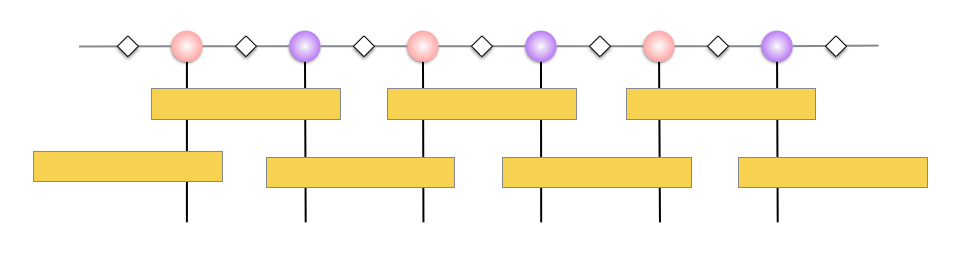
\includegraphics[width=0.90\textwidth]{figures/fig312.png}
	\caption[The tensor diagram of imaginary time evolving block decimation.]{The red and blue tensor denote on \textit{odd} and \textit{even} sites and the yellow tensors are time evolution operators $e^{-\tau H_{AB}}$ and $e^{-\tau H_{BA}}$}
	\label{fig313}
\end{figure}
\section{Infinite Imaginary-Time Evolving Block Decimation for 2-D system}

In this section, we focus on how to implement and optimize 2D-iTEBD algorithms. Interested readers can refer to the related articles for details  \cite{PhysRevLett.99.220405, PhysRevLett.101.090603, PhysRevB.78.155117}.
\label{itebd}
\subsection{One dimensional iTEBD}
To resolve the problem mentioned in the end of the Sec.~\ref{ite}, the "simple update" scheme was developed and have widely applied to iPEPS. 

The tensor diagrams shown in the Fig.~\ref{fig314} are the procedures of 1D-iTEBD which can be simply built by the following steps,
\begin{enumerate}
	\item Initialization: According to Eq. \ref{mapgroud}, the ground state can be obtained from any random state $\Ket{\Psi}$ theoretically. Hence, we provide two rank-3 tensors $\Gamma^{[A]}$ and $\Gamma^{[B]}$ with dimension $dD^2$, where $d$ is the dimension of physical basis and $D$ is the virtual bonds dimension. Two random diagonal matricies $\lambda^{[A]}$ and $\lambda^{[B]}$ are also provided to represent the entanglement between each sites at first. See Fig.~\ref{fig314}(i).
	\item Obtain a cluster tensor $\Theta$: As shown in Fig.~\ref{fig314}(b),
		\begin{enumerate}
			\item Absorb the entangled matrices; 
				\begin{align}
					&\Gamma^{\prime [A]} = \sum_{ij}{\lambda^{[A]}_{i} \Gamma^{A}_{ij \sigma_i} \lambda^{[B]}_{j}} \\
					&\Gamma^{\prime [B]} = \sum_{k}{\Gamma^{B}_{k \sigma_j} \lambda^{[A]}_{k}}
				\end{align}
			\item Utilize the evolution operate $U(\tau)$: The 2-site evolution operator $U(\tau)$ can be simply obtained from Eq. \ref{evoopt}. In this case, 
				\begin{align}
					U(\tau) = e^{-\tau H_{AB}}
				\end{align}
		\end{enumerate}
	\item Decompose $\Theta$ into the general form of MPS: In this step, we utilize singular value decomposition (SVD) to split the tensor $\Theta$ . The SVD decomposition allow to decompose a matrix $A_{m.n}$, with $m \geq n$, into two unitary matrices, $U$, with $m \times m$, and $V^{T}$,with $n \times n$, and an $m \times n$ diagonal matrix $\Sigma$. However, the bottom $m - n$ rows of $\Sigma$ consists only zero elements. Hence, the dimension of $U$ and $\Sigma$ can be reduced,
		\begin{align}
			A = U \Sigma V^T = \begin{bmatrix} U_1 U_2 \end{bmatrix} \begin{bmatrix} \Sigma_1 \\ 0 \end{bmatrix} V^T = U_1 S_1 V^T
		\end{align}
		where $U_1$ is a $m \times n$ unitary matrix, $\Sigma_1$ is a $n \times n$ diagonal matrix. Similarly, when $A_{m,n}$, with $m \leq n$, the matrix $\Sigma_1$ and $V^T$ can be truncated,
\begin{align}
	A = U \Sigma V^T = U \begin{bmatrix} \Sigma_1 0 \end{bmatrix} \begin{bmatrix} V_1^T \\ V_2^T \end{bmatrix} = U \Sigma_1 V_1^T
\end{align}
where $\Sigma_1$ is a $m \times m$ diagonal matrix and $V_1^T$ is a $m \times n$ unitary matrix. There are two significant properties of the singular values term, Assume that,
\begin{align}
\Sigma_1 = diag \left(\sigma_1, \sigma_2, \dots, \sigma_{\max{[m,n]}} \right), 
\end{align}
\begin{enumerate}
	\item All the singular value in $\Sigma_1$ are real.
	\item The singular values are ordered from large to small,
		\begin{align}
			\sigma_1 \geq \sigma_1 \geq \sigma_2 \geq \dots \geq \sigma_{\max{[m,n]}}
		\end{align}
\end{enumerate}
		\item Truncation: See Fig.~\ref{fig314}(iv), we notice that the dimension of bond $j$ increases to $dD$. To avoid the exponential increment of the dimension, the dimension of bond $j$ must be resized to $D$.
		\item Absorb the inverse entangled matrices $\lambda^{[A]}$: Remove the entangle influence from $\widetilde{\Gamma}^{[A]}$ and $\widetilde{\Gamma}^{[B]}$ and return the general form of MPS, as shown in Fig.~\ref{fig314}(v).
			\begin{align}
				&\widetilde{\Gamma}^{[A]} = \sum_{i}{ \lambda_{i}^{[A]^{-1}} \Gamma^{[A]}_{ij,\sigma_i}} \\
				&\widetilde{\Gamma}^{[B]} = \sum_{k}{\Gamma^{[B]}_{jk,\sigma_j} \lambda_{k}^{[A]^{-1}}}
			\end{align}
		\item Repeat the steps (2)-(5) to update the tensors $\widetilde{\Gamma}^{[B]}$, $\widetilde{\Gamma}^{[A]}$ and $\lambda^{[A]}$ with the evolution operator $e^{-\tau H_{BA}}$.
		\item Iterate the steps (2)-(6) until the wave function converges.
\end{enumerate}

\begin{figure}[ht]
	\centering
	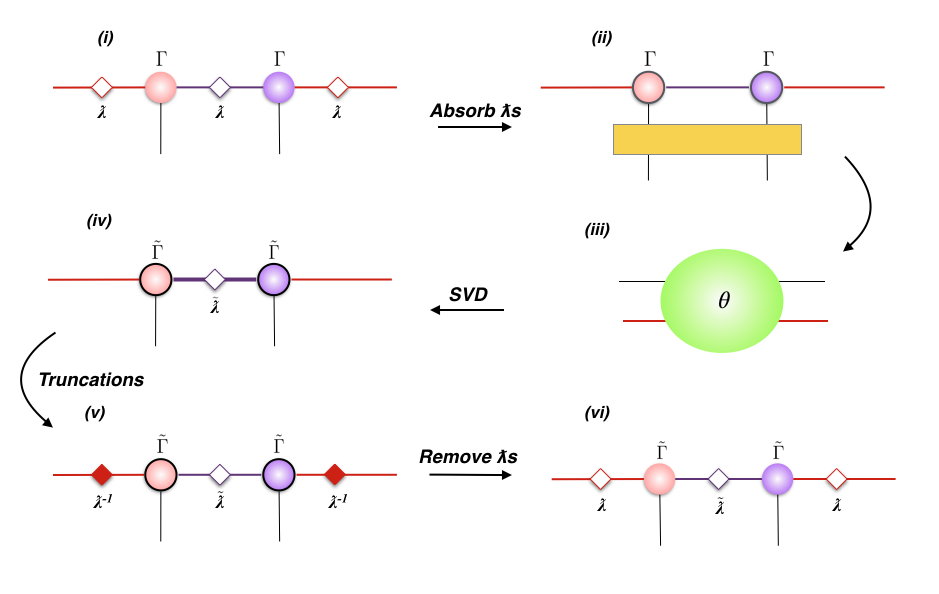
\includegraphics[width=0.90\textwidth]{figures/fig313.png}
	\caption[The tensor network diagrams for the 1-D iTEBD]{ (i)Absorb all $\lambda$ to $\Gamma$. (ii) Contract an evolution operator $e^{-\delta H}$ for evolving the system. (iii) Decompose the tensor $\theta$ by SVD. (iv) Truncate and update the states and $\lambda$ on the green bond.(v) Remove $
		\lambda$ for obtaining the states. (iv) After updating the states and $\lambda$ on the purple bond, we can apply the same way to update the red bond and repeat all the steps until the ground state converges.}
	\label{fig314}
\end{figure}

In one dimensional many-body systems, the performance of iTEBD is good. Although the accuracy is slightly less than DMRG \cite{PhysRevB.48.10345}, it is still widely applied to study or test models due to its high efficiency.

\subsection{Two-dimensional iTEBD}
\label{2ditebd}

Due to the success in one-dimensional cases, we want to extend the framework of iTEBD to simulate two-dimensional systems . In this case, we describe the wave-functions by the projected entangled pair states (PEPS) rather than MPS. 
%%%%%%%%%%%%%%%%%%%%%%%%
The PEPS structure is a straightforward extension of MPS and obeys the restriction of MPS. Therefore, it can be expanded to a infinite structure, iPEPS, which is composed of $n$-site translational invariant states. For instance, we can draw a tensor diagram as shown in Fig.~\ref{fig315} to represent the wave function of a 2-D many-body system which is composed of 2-site translational symmetric states.
%%%%%%%%%%%%%%%%%%%%%%%%

\begin{figure}[ht]

	\centering
	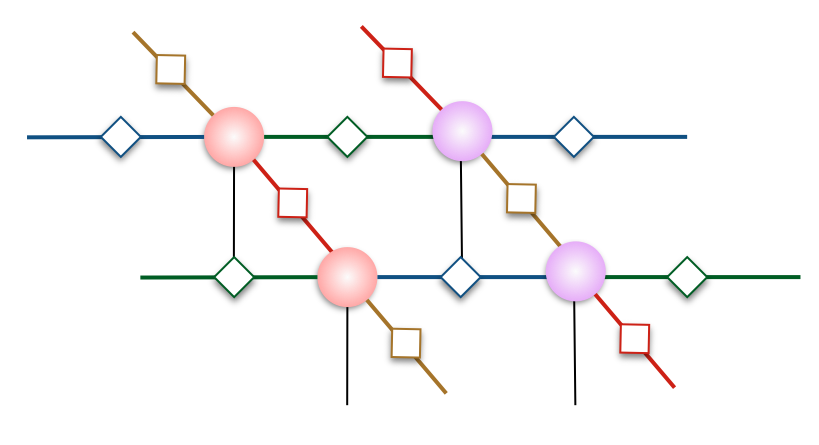
\includegraphics[width=0.6\textwidth]{figures/fig314.png}
	\caption[The tensor diagrams of 2-D lattice]{Four sites unit cell in iPEPS.}
	\label{fig315}
\end{figure}

The most intuitive update method is directional simple update, which means that the states of iPEPS must be updated by iTEBD along four directional moves: namely up, right, down and left. The scheme of implementing 2D-iTEBD is shown as follows which starts from the right move,

\begin{enumerate}
	\item Initialization: To describe iPEPS states [Fig.~\ref{fig316}], we need two random rank-5 tensors $\Gamma^{[A]}_{uldr,\sigma_j}$ and $\Gamma^{[B]}_{uldr, \sigma_j}$ with dimension $dD^4$, and four random diagonal matrices $\lambda_{u}$, $\lambda_{l}$, $\lambda_{d}$ and $\lambda_{r}$.
	\item Obtain a cluster tensor $\Theta$: As shown in Fig.~\ref{fig315}(ii),
		\begin{enumerate}
			\item Absorb the entangled matrices; 
				\begin{align}
					&\Gamma^{\prime [A]}_{uldr,\sigma_i} = \sum_{uldr}{ \lambda_{u}\lambda_{l} \Gamma^{[A]}_{ulrd,\sigma_i} \lambda_{r} \lambda_{d}} \\
					&\Gamma^{\prime [B]}_{uldr,\sigma_j} = \sum_{uld}{\lambda_{d} \Gamma^{B}_{uldr,\sigma_j} \lambda_{u}\lambda_{l}}
				\end{align}
			\item Utilize the evolution operate $U(\tau)$: See Fig.~\ref{fig316}(iii)
				\begin{align}
					\Theta = \sum_{r,\sigma_i^{\prime}\sigma_j^{\prime}}{U^{\sigma_i^{\prime}\sigma_j^{\prime}}_{\sigma_i\sigma_j} \Gamma^{\prime\sigma_i [A]}_{uld,r} \Gamma^{\prime \sigma_j[B]}_{r,u^{\prime} l^{\prime} d^{\prime}}}
				\end{align}
				the rank of $\Theta$ is eight and the dimension is $d^2D^6$.
			\end{enumerate}
		\item Decompose $\theta$ into the general form of iPEPS:
		\item Truncation: See Fig.~\ref{fig316}(iv), the dimension of bond $r$ increases to $dD^3$. To reduce the computational consumption, we must truncate the dimension to a smaller $D$.
		\item Absorb the inverse entangled matrix surrounding $\Gamma^{\prime [A]}$ and $\Gamma^{\prime [B]}$: Return to the general form of the iPEPS, as shown in Fig.~\ref{fig316}(v).
				\begin{align}
					&\widetilde{\Gamma}^{[A]}_{uldr,\sigma_i} = \sum_{uldr}{ \lambda_{u}^{-1} \lambda_{l}^{-1} \Gamma^{[A]}_{ulrd,\sigma_i} \lambda_{d}^{-1}} \\
					&\widetilde{\Gamma}^{[B]}_{uldr,\sigma_j} = \sum_{uld}{\lambda_{d}^{-1} \Gamma^{[B]}_{uldr,\sigma_j} \lambda_{u}^{-1} \lambda_{l}^{-1}}
				\end{align}
			\item Repeat the steps (2)-(5) to update the other directional moves. To explain more explicitly, the procedures of the up move are shown in Fig.~\ref{fig317}.
			\item Iterate the steps (2)-(6) until the wave-function converges.
			
\end{enumerate}

\begin{figure}[ht]
	\centering
	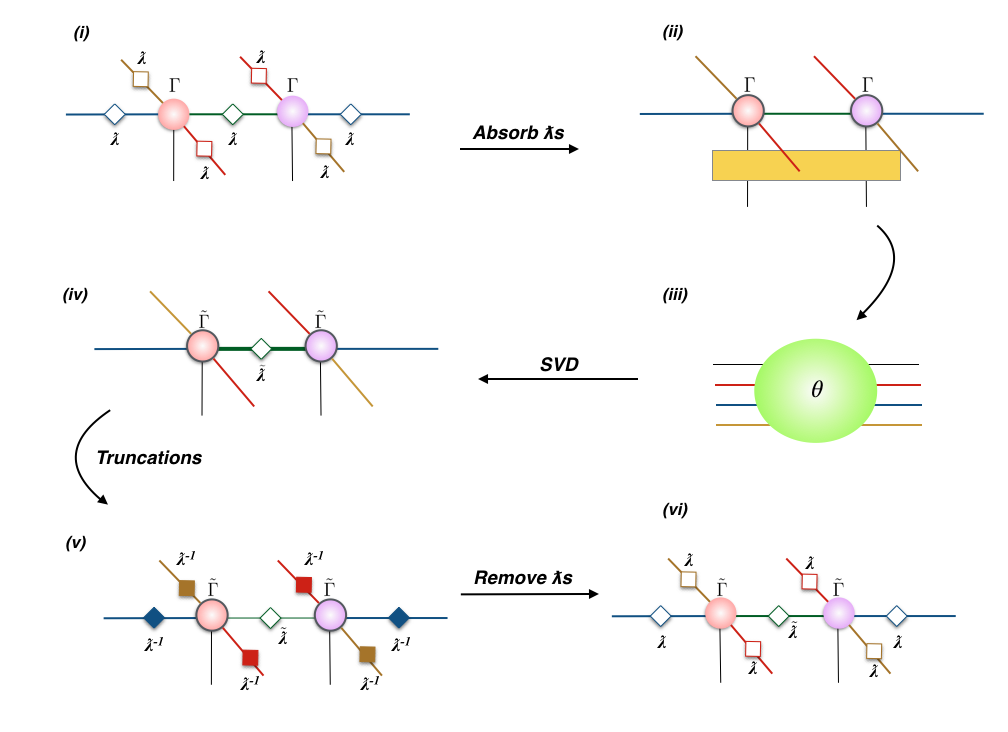
\includegraphics[width=0.80\textwidth]{figures/fig315.png}
	\caption[The tensor network diagrams of updating the green bond in iPEPS with 2D-iTEBD]{Absorb all $\lambda$ to $\Gamma$. (ii) Contract an evolution operator $e^{-\delta H}$ for evolving the system. (iii) Decompose the tensor $\theta$ by SVD. (iv) Truncate and update the states and $\lambda$ on the green bond.(v) Remove $\lambda$ for obtaining the states. (iv) Obtain a original form of iPEPS. Repeat all the step to update the other bonds until the ground state energy converges}
	\label{fig316}
\end{figure}

	\begin{figure}[ht]
	\centering
	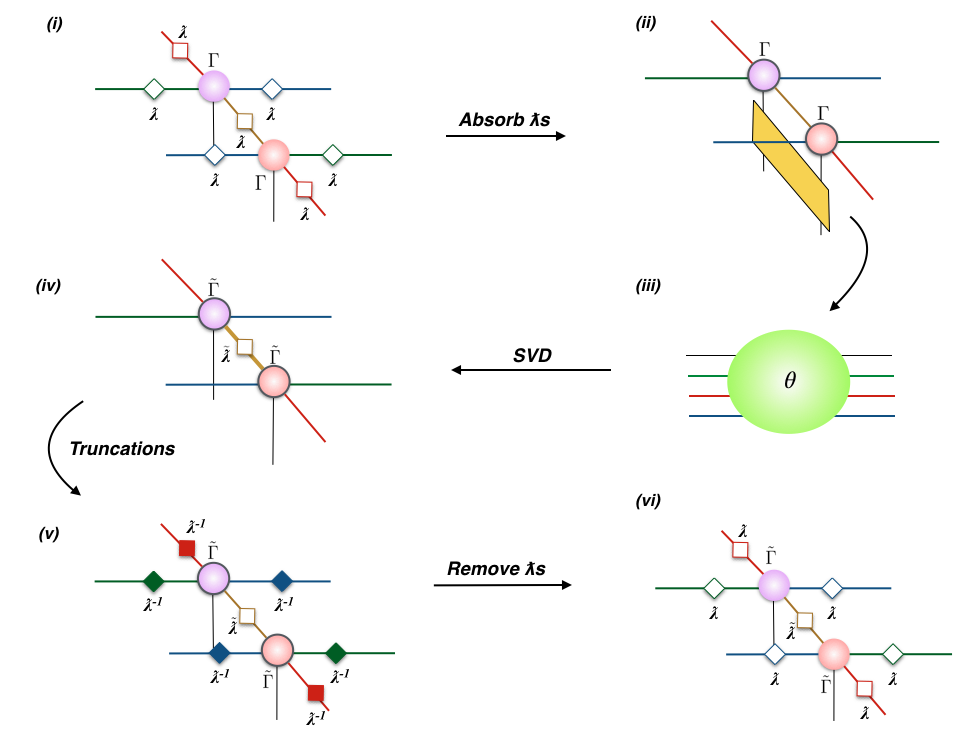
\includegraphics[width=0.80\textwidth]{figures/fig316.png}
	\caption[The tensor network diagrams of updating the yellow bond in iPEPS with 2D-iTEBD]{Update the yellow bond and the steps are similar to Fig.\ref{fig315}}
	\label{fig317}
	\end{figure}

\section{Improvement a la Hastings}
\label{2dhastin}

The directional simple update discussed in Sec.~\ref{2ditebd} can give good iPEPS states in simple models. However, in some complicated models it becomes unstable and inefficient. The reason is that there are too many multiplications of pseudo-inverse $\lambda^{-1}$ at the step Fig.\ref{fig316}(v). In numerical methods, it is dangerous to divide a value by a number which is equal or approach to zero. In other words, the more inverse operations, the more probability of numerical instability. Hence, Hastings developed another scheme to improve that the stability \cite{light_hastings}. The procedures from the right is shown as follows,

\begin{enumerate}
	\item Initialization: As in the directional simple update, we generate two random $\Gamma^{[A]}$ and $\Gamma^{[B]}$, and four random diagonal matrices $\lambda_{u}$, $\lambda_{r}$, $\lambda_{l}$ and $\lambda_{d}$ to describe the wave function. However, the definition of $\Gamma^{[A]}$ and $\Gamma^{[B]}$ are different. In this scheme,
		\begin{align}
			\Gamma^{[A]}_{ulrd,\sigma_i} \equiv \sum_{ur}{\lambda_{u} \Gamma^{[A_s]}_{ulrd,\sigma_i} \lambda_{r}} \\
			\Gamma^{[B]}_{ulrd,\sigma_j} \equiv \sum_{dl}{\lambda_{d} \Gamma^{[B_s]}_{ulrd,\sigma_j} \lambda_{l}}
		\end{align}
		where $\Gamma^{[A_s]}_{ulrd,\sigma_i}$ and $\Gamma^{[B_s]}_{ulrd,\sigma_j}$ are the definition in directional simple update. [In sec.\ref{2ditebd}].
	\item Obtain the cluster tensor $C$: As shown in Fig.~\ref{fig318}(b),
			\begin{enumerate}
				\item Absorb the entangled matrices $\lambda_{u}$ into  $\Gamma^{[B]}_{ulrd,\sigma_j}$:
					\begin{align}
						%&\Gamma^{\prime [A]}_{uldr, \sigma_j} = \sum_{dl}{\lambda_{i} \Gamma^{A}_{ij \sigma_i} \lambda_{j}} \\
						&\Gamma^{\prime [B]}_{uldr, \sigma_j} = \sum_{u}{\Gamma^{[B]}_{uldr,\sigma_j} \lambda_{u}}
					\end{align}
				\item Contract the tensors $\Gamma^{[A]}$, $\Gamma^{\prime [B]}$ and the evolution operate $U(\tau)$: 
					\begin{align}
						C = \sum_{r,\sigma_i^{\prime}\sigma_j^{\prime}}{U^{\sigma_i^{\prime}\sigma_j^{\prime}}_{\sigma_i\sigma_j} \Gamma^{\sigma_i [A]}_{uld,r} \Gamma^{\prime \sigma_j[B]}_{r,u^{\prime} l^{\prime} d^{\prime}}}
					\end{align}
			\end{enumerate}
		\item Obtain the cluster tensor $\Theta$: In the step, the entanglement surrounding $\Gamma^{[A]}$ would be absorbed in the tensor $C$,
			\begin{align}
				\Theta = \sum_{dl}{\lambda_{d} \lambda_{l} C^{udl,\sigma_i}_{u^{\prime}d^{\prime}l^{\prime},\sigma_j}}
			\end{align}
		\item Decompose $\theta$ into the general form of the iPEPS and truncate the updated bond: This step is same as directional simple update, see Fig.~\ref{fig318}(v).
		\item Update $\Gamma^{[A]}$: Due to the tensor $C$ does not contain the entanglement surrounding $\Gamma^{[A]}$, the updated $\Gamma^{[A]}$ can be obtained by contracting tensors $C$ and $\widetilde{\Gamma}^{[B]}$
			\begin{align}
				\Gamma^{[A]} = \sum_{u^{\prime}l^{\prime}r^{\prime}\sigma_j}{C^{udl,\sigma_i}_{u^{\prime}d^{\prime}l^{\prime},\sigma_j} \widetilde{\Gamma}^{\sigma_j [B]}_{u^{\prime}d^{\prime}l^{\prime}}}
			\end{align}
		\item Absorb the inverse $\lambda_{u}$ into $\widetilde{\Gamma}^{[B]}_{ulrd,\sigma_j}$:
			\begin{align}
				\Gamma^{[B]} = \sum_{u}{\lambda_{u}^{-1}\widetilde{\Gamma}^{[B]}_{ulrd,\sigma_j}}
			\end{align}
			, which is shown as Fig.~\ref{fig318}.
		\item Repeat the steps (2)-(5) to update the others directional moves, down, left and up.  
		\item Iterate the steps (2)-(6) until the wave function converges.
\end{enumerate}

In the procedures of directional simple update, there are six pseudo-inverse $\lambda^{-1}$ must be absorbed in each iteration. Relatively, in this scheme we just need to multiply a pseudo-inverse $\lambda^{-1}$ in step(6). Nevertheless, the computational cost of updating states in step(5) is higher than the update in directional simple update and take more time in each iteration. Numerical stability makes the wave function converge with less iterations.

\begin{figure}[ht]
	\centering
	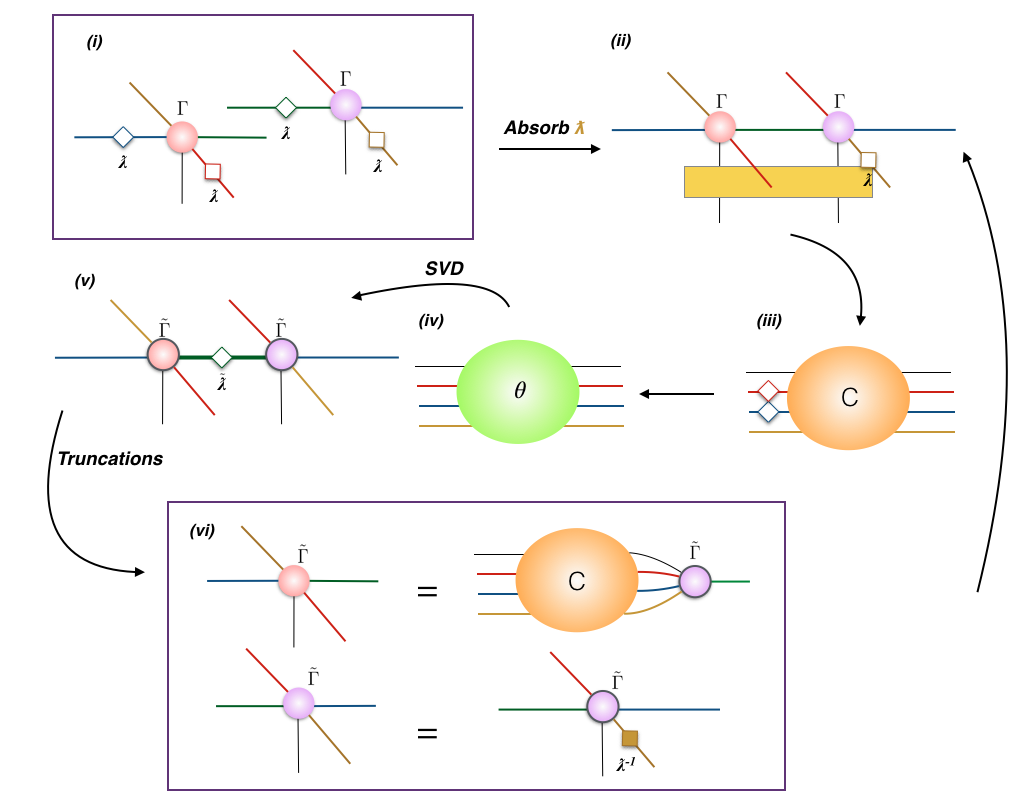
\includegraphics[width=1.00\textwidth]{figures/fig317.png}
	\caption[The tensor network diagrams for the 2-D iTEBD with QR decomposition]{The tensor network diagrams for the improve 2-D iTEBD.}
	\label{fig318}
\end{figure}

\section{Optimizations}
\label{2dopt}

\subsection{Initialization}
\label{2doptInit}

Theoretically, regardless of which initial state we use, the ground state wave-function can be obtained by iTEBD algorithms. However, many trials show that starting from an bad initial state might cause the break down the algorithms. Hence, we need to "guess" a good initial state.

\begin{enumerate}
	\item Begin from product states.
	\item Consider the translational invariance: For example, there is a iPEPS shown as Fig.~\ref{fig321}(i). The arrangement of coefficients in the states $A_{hurdl}$ should be the same as $B_{hdlur}$, see Fig.~\ref{fig321}(ii).
\end{enumerate}

\begin{figure}[ht]
	\centering
	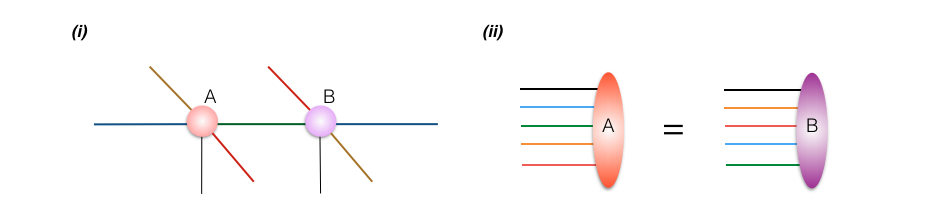
\includegraphics[width=1.00\textwidth]{figures/fig321.png}
	\caption[The diagrams of initializing projected entangled pair states]{(i) The structure of PEPS, (ii) The initialization of states}
	\label{fig321}
\end{figure}

\subsection{QR and LQ decomposition}
\label{2doptQR} 
In Sec.~\ref{2ditebd} and Sec.~\ref{2dhastin}, we introduced two different methods to implement 2D-iTEBD. However, it is hard to apply them when the dimension of the virtual bonds becomes larger due to the rapid increment of the dimension of tensor $\Theta$ [Fig.~\ref{fig316}(iii) and Fig.~\ref{fig318}(iii)] which is a rank-8 tensor with dimension $d^2D^6$. In addition to the problem of the consumption, the singular value decomposition, is expensive because the time complexity is proportional to $O(M^2N)$. Therefore, in this section we apply QR and LQ decomposition to reduce the rank of $\Theta$.

The QR decomposition decomposes a real or complex matrix $A_{m,n}$, with $m \geq n$, into a $m \times m$ unitary matrix $Q$ and a $m \times n$ upper triangular matrix $R$. However, in bottom $(m-n)$ rows of $R$ are filled with zeros. Hence, the matrix $Q$ and $R$ can be truncated,
\begin{align}
	A = QR = Q \begin{bmatrix} R_1 \\ 0 \end{bmatrix} = \begin{bmatrix} Q_1, Q_2 \end{bmatrix} \begin{bmatrix} R_1 \\ 0 \end{bmatrix} = Q_1 R_1, 
\end{align}
where $Q_1$ is a $m \times n$ unitary matrix and $R_1$ is a $(n \times n)$ upper triangular matrix. Analogously, the LQ decomposition can decompose a matrix $A_{m,n}$, with $m \leq n$ into a $m \times m$ lower triangular matrix $L_1$ and a $m \times n$ unitary matrix $Q_1$, 
\begin{align}
	A = LQ = \begin{bmatrix} L_1, 0 \end{bmatrix} Q = \begin{bmatrix}  L_1, 0\end{bmatrix} \begin{bmatrix} Q_1 \\ Q_2 \end{bmatrix} = L_1 Q_1, 
\end{align}

In the case of the directional simple update, most of the steps of implementing with QR decomposition is similar to original one, see Fig.~\ref{fig319}. There exists only two differences, 
\begin{enumerate}
	\item After the entangled matrices $\lambda$s are absorbed, we decompose the states $\Gamma^{[A]}$ into a unitary matrix $X$ and a upper triangular matrix $a_R$,
		\begin{align}
			\Gamma^{[A]}_{\chi_d \chi_l \chi_u, \chi_{\sigma_i} \chi_r} = X_{\chi_d \chi_l \chi_u, \chi_{\sigma_i} \chi_r} {a_R}_{\chi_{\sigma_i} \chi_r,\chi_{\sigma_i} \chi_r}
		\end{align}
		and decompose $\Gamma^{[A]}$ into a unitary matrix $Y$ and a lower triangular matrix $b_L$
		\begin{align}
			\Gamma^{[B]}_{\chi_{\sigma_j} \chi_r, \chi_d \chi_l \chi_u} = {b_L}_{\chi_{\sigma_j} \chi_r,\chi_{\sigma_j} \chi_r} Y_{\chi_{\sigma_i} \chi_r, \chi_d \chi_l \chi_u} 
		\end{align}
		where $\chi_n$ means the dimension of the bond $n$. See Fig.~\ref{fig319}(ii).
	\item Contract $X$ and $a_R$ into $\Gamma^{[A]}$ and $b_L$ and $Y$ into $\Gamma^{[B]}$ before the inverse matrices are absorbed. See Fig.~\ref{fig319}(v).

\end{enumerate}
\begin{figure}[H] 
	\centering 
	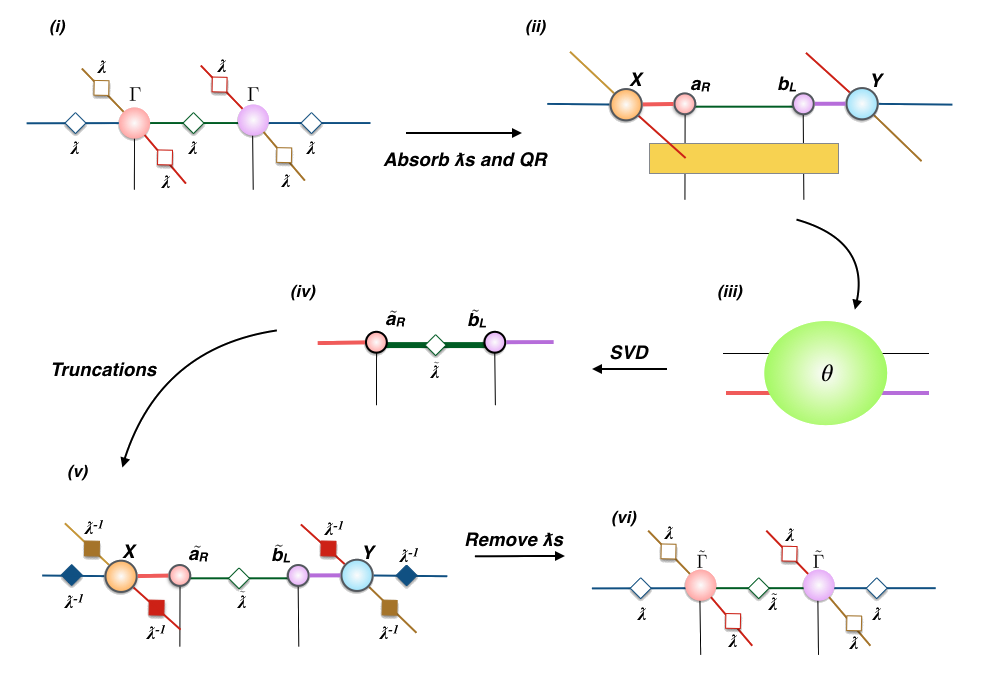
\includegraphics[width=1.00\textwidth]{figures/fig318.png} 
	\caption[The tensor network diagrams for the improve 2-D iTEBD with QR decomposition]{The tensor network diagrams for the improve 2-D iTEBD with QR and LQ decomposition.} 
	\label{fig319} 
\end{figure} 

\begin{figure}[!ht]
	\centering
	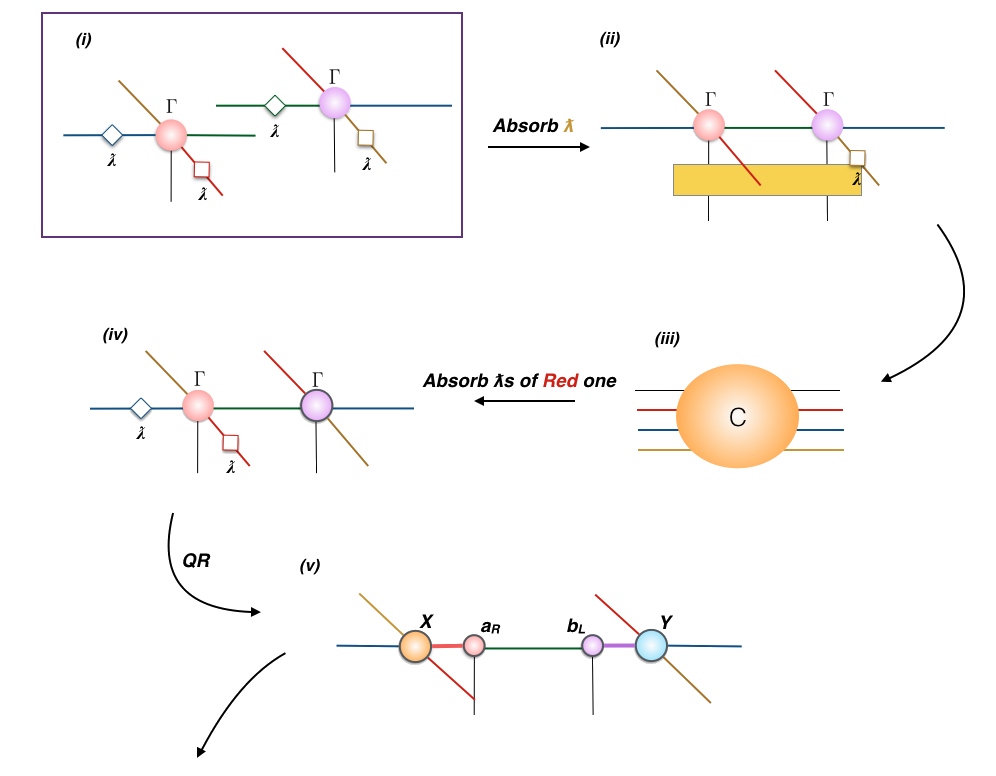
\includegraphics[width=1.00\textwidth]{figures/fig319.png}
	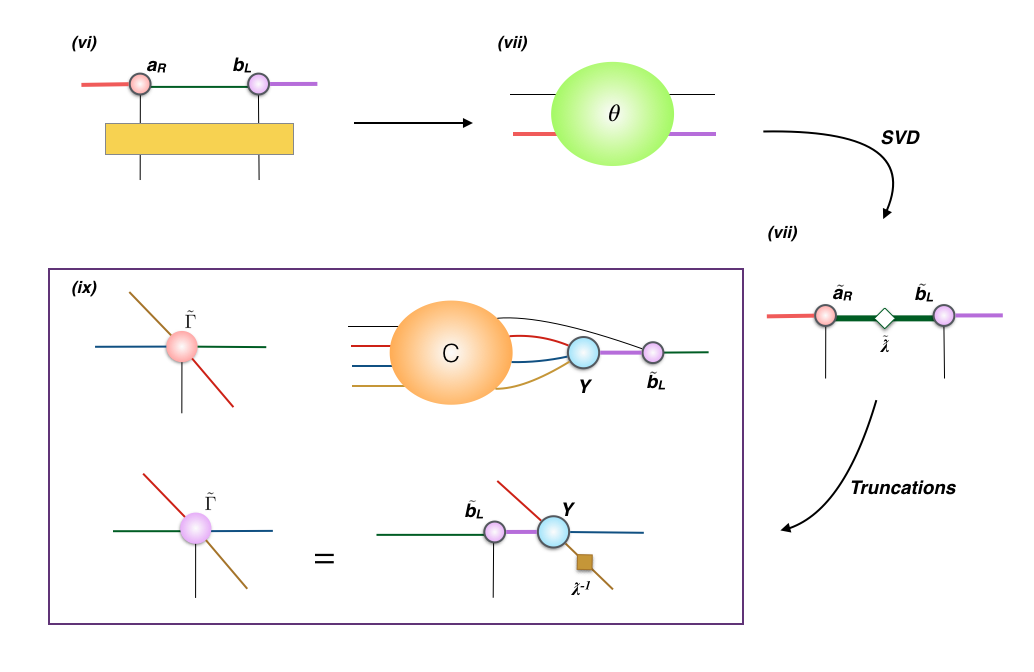
\includegraphics[width=1.00\textwidth]{figures/fig320.png}
	\caption[The tensor network diagrams for the improve 2-D iTEBD with QR and LQ decomposition]{The tensor network diagrams for the improve 2-D iTEBD with QR and LQ decomposition.}
	\label{fig320}
\end{figure}

Nevertheless, the main idea to reduce the tensor $\Theta$ in ameliorate 2D-iTEBD in the same way as the directional simple update. The scheme becomes more complicated, see Fig.~\ref{fig320}, 

\begin{enumerate}
	\item Instead absorb $\lambda_d$ and $\lambda_l$ into the cluster tensor $C$, we absorb them into $\Gamma^{[A]}$
		\begin{align}
			\Gamma^{\prime [A]}_{uldr,\sigma_i} = \sum_{dl}{\lambda_l \Gamma^{[A]}_{uldr,\sigma_i} \lambda_d}
		\end{align}
		and apply the QR and LQ decomposition to split $\Gamma^{\prime [A]}$ and $\Gamma^{\prime [B]}$ into $X\cdot a_R$ and $b_L \cdot Y$. See Fig.~\ref{fig320}(iv) and Fig.~\ref{fig320}(v) 
	\item Obtain $\widetilde{\Gamma}^{[A]}$ by contracting tensor $C$, $Y$ and $b_L$, as shown in Fig.~\ref{fig320}(ix)
		\begin{align}
			\widetilde{\Gamma}^{[A]}_{urld, \sigma_i} = \sum_{u^{\prime}l^{\prime}d^{\prime}\sigma_j,q}{C^{dlu\sigma_i}_{d^{\prime}l^{\prime}u^{\prime}\sigma_i}Y_{d^{\prime}l^{\prime}u^{\prime}q}{b_L}_{qr}}
		\end{align}
		and obtain $\widetilde{\Gamma}^{[B]}$ by contracting $Y$, $b_L$ and $\lambda_u^{-1}$
		\begin{align}
			\widetilde{\Gamma}^{[B]}_{urld,\sigma_j} = \sum_{q}{{b_L}_{rq}Y_{uld\sigma_j q}\lambda_u^{-1}}
		\end{align}
\end{enumerate}

After these operations, the clustered tensor $\Theta$ is reduced to a rank-4 tensor, with dimension $d^2D^2$.

\subsection{Truncation Error}
\label{truncaterr}
In order to control the increase virtual bond dimensions, we must truncate the updated bond from $dD^3$ or $d^2D$ to $D$ after decomposing the tensor $\Theta$. However, if the singular values contained in $\Sigma$ are not concentrated to the leading terms, some influential features and basis would be dropped and the algorithms might be broken. Therefore, we set a cutoff $\varepsilon$, 
\begin{align}
	\varepsilon \geq 1 - \sum_{i=1}^{\chi}{\sigma_i^2}
\end{align}
to determine the dimension of the updated bond, where $\sigma_i$ is the elements at $\Sigma_{[i,i]}$ and $\chi$ is the number of the remained basis . However, it doesn't mean that better accuracy with smaller $\varepsilon$ because setting a smaller cutoff also implies that more basis states and close-to zero singular values in $\Sigma$ are kept. A proper choice of $\varepsilon$ is important.

\section{Comparison} 
\label{Comparison}

Now we compare the results for the Heisenberg model on the square lattice,
\begin{align}
	\label{mapgroud}
	H = J \sum_{<ij>}{\left( S^{x}_{i}S^{x}_{j}+S^{y}_{i}S^{y}_{j}+S^{z}_{i}S^{z}_{j} \right)}
\end{align}
and show the effect of the various optimizations.

\subsection{Different Initializations}

\begin{figure}[ht]
	\centering
	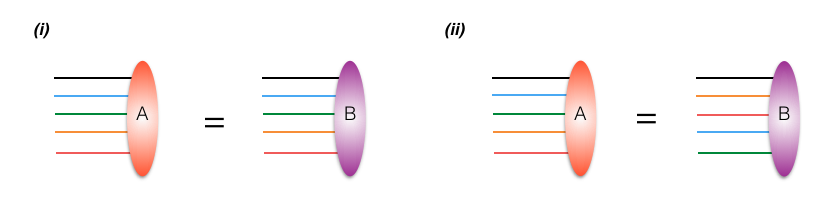
\includegraphics[width=1.00\textwidth]{figures/fig322.png}
	\caption[Different methods to initialize the states]{(i) Type 1, (ii) Type 2}
	\label{fig322}
\end{figure}

Assume that the iPEPS states are constructed as Fig.~\ref{fig321}(i) and the algorithm starts from two different initial states, see Fig.~\ref{fig322}(i) and Fig.~\ref{fig322}(ii). Obviously, The Type1 method does not obey translational symmetry. Hence, the algorithm might hardly converge or even break down. As shown in Fig \ref{fig323}, the efficient ameliorate 2D-iTEBD (Hastings+QR) starting from the initial states which are obtained from Type2 [Fig.~\ref{fig322}(ii)] converge in less 1000 epochs. However, if we begin from the Type1 states [Fig.~\ref{fig322}(i)], the algorithm does not converge in 7000 epochs and even be broken in the end. 
In conclusion, through many experiment we have known that this problem may not only occur in 2D-iTEBD, but also in any algorithm which is based on the theory of imaginary-time evolution, such as fast full update \cite{PhysRevB.92.035142}, PESS \cite{PhysRevX.4.011025}.

\begin{figure}[ht]
	\centering
	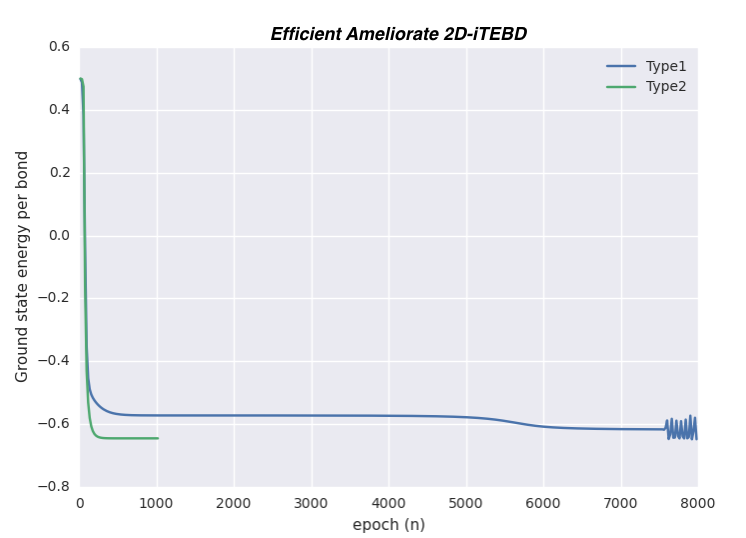
\includegraphics[width=0.75\textwidth]{figures/fig323.png}
	\caption[Comparison the results of Heisenberg model on square lattice which are obtaining from different initial states.]{Comparison the results of Heisenberg model on square lattice are obtaining from different initial states. The Blue line represents updating tensors from the initial state shown in Fig \ref{fig322} (i) and the green one represents updating from Fig \ref{fig322} (ii)}

	\label{fig323}
\end{figure}

\subsection{Different schemes of 2D-iTEBD}

In previous sections, we have introduced four different implementations of 2D-iTEBD, \textit{Simple Update}, \textit{Ameliorate Simple Update}, \textit{Simple Update with QR decomposition} and \textit{Ameliorate Simple Update with QR}. In Fig.~\ref{fig325}, we notice that the methods based on Hastings scheme are more stable than the other which are build on \textit{Simple Update}. The Hastings ways can converge rapidly in 1,000 epochs. However, due to multiplying too many pseudo-inverse matrices, the other methods can not converge in 10,000 epochs, and break down in the end. Nevertheless, according to the result shown in Fig.~\ref{fig325}, we find that the QR decomposition has no effects on the stability but it makes the algorithms more efficient, see Fig.~\ref{fig324}. Due to the reduced dimensions of the tensor $\Theta$, the time cost does not increase exponentially with virtual bond dimensions. Therefore, we can simply study the two dimensional systems with a sufficient large virtual bond dimension $D$, which means that we can obtain the better ground states more quickly and the measurement can be calculated more accurately with larger $D$.

\begin{figure}[ht]
	\centering
	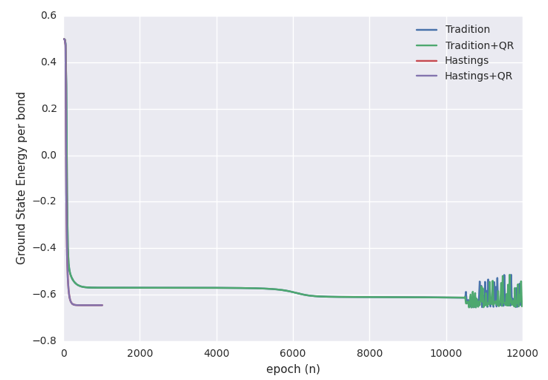
\includegraphics[width=0.70\textwidth]{figures/fig325.png}
	\caption[Comparison the efficiency of various 2D-iTEBD]{Comparison the efficiency of various 2D-iTEBD with fixed truncation error.}
	\label{fig325}
\end{figure}

\begin{figure}[ht]
	\centering
	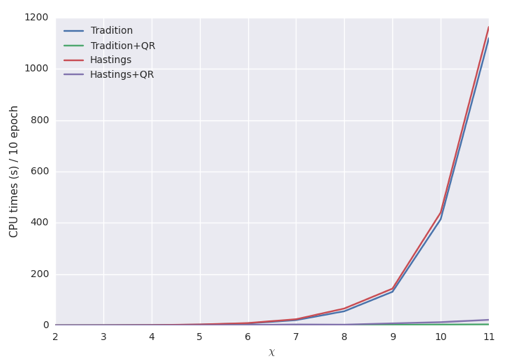
\includegraphics[width=0.70\textwidth]{figures/fig324.png}
	\caption[Compare CPU times per 10 epochs of different 2D-iTEBD with fixed trucation error]{Compare CPU times per 10 epochs of different 2D-iTEBD with fixed truncation error}
	\label{fig324}
\end{figure}

\section{Cutoff of the truncation error}

To improve the stability of the algorithms, we can set a cutoff $\varepsilon$ of the truncation error. In Fig.~\ref{fig326}, we set $\varepsilon = 10^{-7}$ and the methods based on traditional simple update would not be broken and converge in 2300 epochs. Intuitively, a smaller cutoff leads to more accurate ground states. However, it is inefficient and unnecessary. As shown in Fig.~\ref{fig327}, to prevent from the breaking of the algorithms, the required virtual bond dimension increase to an large scale. As a result, this approach requires mush computational effort but its performance is still inefficient and unstable. 

\begin{figure}[ht]
	\centering
	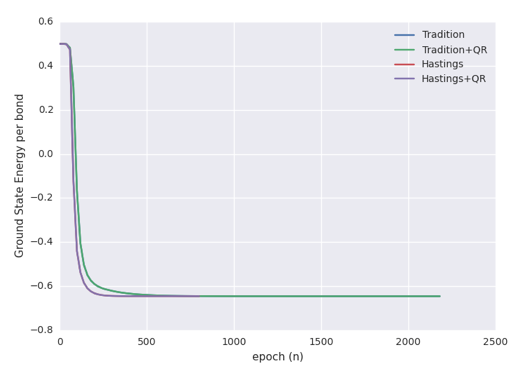
\includegraphics[width=0.65\textwidth]{figures/fig326.png}
	\caption[Energy per epoch of Heisenberg model on two-dimensional square lattice with the cutoff, $\varepsilon = 10^{-7}$]{Per epoch energy of Heisenberg model on two-dimensional square lattice with the cutoff, $\varepsilon = 10^{-7}$.}
	\label{fig326}
\end{figure}

\begin{figure}[ht]
	\centering
	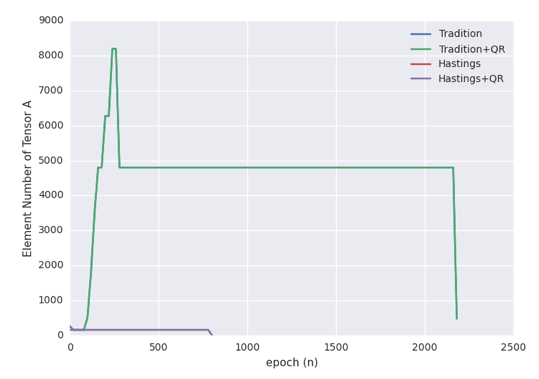
\includegraphics[width=0.65\textwidth]{figures/fig327.png}
	\caption[The requirement of the virtaul bond dimension with the cutoff of the truncation error $\varepsilon = 10^{-7}$]{The requirement of the virtual bond dimension with the cutoff of the truncation error $\varepsilon = 10^{-7}$.}
	\label{fig327}
\end{figure}
